\documentclass[10pt]{article}
\usepackage[margin=0.78in]{geometry}
\usepackage{amsmath,amssymb}
\usepackage{booktabs}
\usepackage{graphicx}
\usepackage{xcolor}
\usepackage[hidelinks]{hyperref}
\usepackage{microtype}
\usepackage{enumitem}
\setlist{nosep,leftmargin=*}
\newcommand{\R}{\mathbb{R}}
\newcommand{\E}{\mathbb{E}}
\newcommand{\N}{\mathcal{N}}
\title{Action-Conditioned Neural Likelihood Learning\\for Stochastic Wireless Simulators}
\author{Wireless Neural Likelihoods Contributors}
\date{August 2026}

\begin{document}
\maketitle

\begin{abstract}
Wireless adaptation requires a probabilistic account of what a receiver may observe under a channel state and a proposed communication action. Analytical likelihoods are often unavailable once temporal correlation, bursts, interference, and receiver behavior interact. We present an open, reproducible Python implementation that learns the conditional density of continuous receiver telemetry from simulations. The repository contains five stochastic channel families, three structured actions, a receiver abstraction, family-specific and joint three-component Gaussian mixture density networks, grouped state splits, and Bayesian updating utilities. We compare five family-specific networks against one family-conditioned joint network over 30 independent seeds. On held-out channel states, the joint network improves macro-average negative log likelihood (NLL) by 0.0799, with a 95\% confidence interval of $[0.0595,0.1002]$, and wins on 96.7\% of seeds. Mean paired gains are positive for all five families, with the largest gain on log-Gaussian fading. These results support joint amortization for the tested simulator collection, while also showing where calibration tests and higher-fidelity receiver backends are needed.
\end{abstract}

\section{Introduction}

A simulator can generate realistic observations even when its probability density cannot be evaluated. This creates a practical inverse problem: given receiver telemetry, how should a system evaluate or infer the channel state that could have produced it? Simulation-based inference (SBI) addresses this setting by learning a density or density ratio from simulator draws \cite{cranmer2020frontier}. Neural likelihood estimation learns a conditional density that can be reused with priors, sequential observations, and standard Bayesian computations.

This repository develops a small but complete test bed for wireless neural likelihood learning. It is deliberately positioned between a toy regression example and a waveform-level link simulator. The channel backends expose different temporal structures, while a common receiver interface produces action-dependent telemetry. The learned object is a normalized density, not only a point prediction:
\begin{equation}
  q_{\phi}(m\mid\theta,a) \approx p_{\mathrm{sim}}(m\mid\theta,a),
  \label{eq:objective}
\end{equation}
where $\theta$ is a channel-state vector, $a$ is a structured communication action, $m$ is observed receiver telemetry, and $\phi$ denotes neural-network parameters. Equation~\eqref{eq:objective} makes the output useful in a Bayesian update and allows held-out NLL to compare predictive distributions.

The main contributions are:
\begin{itemize}
  \item a reproducible simulator-to-inference software path covering IID errors, a Gilbert--Elliott process, fixed bursts, ON/OFF Markov interference, and RBF-correlated log-Gaussian fading;
  \item conditional Gaussian and Gaussian-mixture neural likelihoods that use explicit channel-state and action features;
  \item a leakage-resistant evaluation protocol that assigns entire channel-state points, including all their stochastic replicates, to training, validation, or test;
  \item a 30-seed paired comparison of separate and joint likelihood learners, with Student-$t$ confidence intervals, paired tests, and raw per-seed results; and
  \item a literature-vetted connection between SBI methodology and data-driven wireless channel modeling.
\end{itemize}

The report first defines the simulated system and the learned density, then describes implementation and evaluation, presents repeated-seed results, relates the work to prior research, and closes with limitations and extensions.

\section{System and Measurement Model}

\subsection{Simulation interface}

For a chosen family, the simulator draws a raw frame outcome
\begin{equation}
  x \sim p_{\mathrm{ch}}(x\mid\theta,a), \qquad
  m \sim p_{\mathrm{rx}}(m\mid x,a).
  \label{eq:simulator}
\end{equation}
Here $x$ includes a 64-symbol binary error sequence and optional latent diagnostics. The receiver map produces the telemetry $m$. The present channel simulators do not directly depend on $a$; action dependence enters through the receiver. Writing $a$ in both factors in Equation~\eqref{eq:simulator} preserves an interface that can later support action-dependent physical simulations.

Table~\ref{tab:channels} lists the sampled state variables. Every state is drawn independently from the displayed ranges for each experimental seed.

\begin{table}[t]
\centering
\small
\caption{Channel families and sampled state ranges. Lengths are in symbols.}
\label{tab:channels}
\begin{tabular}{p{0.19\linewidth}p{0.71\linewidth}}
\toprule
Family & State parameters and ranges \\
\midrule
IID error & error probability $p_e\in[0.001,0.3]$ \\
Gilbert--Elliott & $p_{G\to B}\in[0.005,0.08]$, $p_{B\to G}\in[0.08,0.4]$, $p_e^G\in[0.001,0.03]$, $p_e^B\in[0.12,0.45]$ \\
Fixed burst & background error $[0.002,0.04]$, burst probability $[0.01,0.5]$, burst length $[2,16]$, burst error $[0.15,0.55]$ \\
Markov interference & OFF-to-ON $[0.01,0.15]$, ON-to-OFF $[0.08,0.4]$, OFF error $[0.001,0.03]$, ON error $[0.12,0.5]$ \\
Log-Gaussian fading & mean log-SNR $[-0.2,1.5]$, log-SNR standard deviation $[0.15,0.8]$, correlation length $[2,21.33]$, SNR offset $[0.8,1.5]$ \\
\bottomrule
\end{tabular}
\end{table}

The Gilbert--Elliott and interference simulators initialize their binary latent Markov states from the stationary distribution. The fixed-burst model adds at most one contiguous high-error segment to an IID background. For the fading model, latent log-SNR values $s_1,\ldots,s_T$ have covariance
\begin{equation}
  \operatorname{Cov}(s_i,s_j)=\sigma_s^2
  \exp\!\left[-\frac{(i-j)^2}{2\ell^2}\right],
  \label{eq:rbf}
\end{equation}
where $\sigma_s$ controls fading variation and $\ell$ controls temporal smoothness. The resulting error probability is a bounded logistic function of linear-scale SNR. Thus Equation~\eqref{eq:rbf} supplies temporal correlation without claiming to reproduce waveform propagation.

\subsection{Actions and receiver telemetry}

An action is represented by four numeric features: redundancy, interleaver depth, receiver-algorithm strength, and computation budget. The three defaults are shown in Table~\ref{tab:actions}. Their generic semantics make the likelihood interface independent of a particular coding implementation.

\begin{table}[h]
\centering
\small
\caption{Default structured actions.}
\label{tab:actions}
\begin{tabular}{lrrrr}
\toprule
Action & Redundancy & Interleaver & Strength & Budget \\
\midrule
Fast, low redundancy & 0.10 & 1 & 0.7 & 0.5 \\
Interleaved & 0.20 & 8 & 1.0 & 1.0 \\
Robust & 0.35 & 16 & 1.5 & 2.0 \\
\bottomrule
\end{tabular}
\end{table}

The abstract receiver converts raw error rate $e$, burst fraction $b$, and a transition-derived correlation proxy $c$ into a noisy difficulty
\begin{equation}
 d = 10e+1.2b+0.35c-3r-0.8s-0.4\log(1+i)+\epsilon_d,
 \label{eq:difficulty}
\end{equation}
where $(r,i,s)$ are redundancy, interleaver depth, and strength, and $\epsilon_d\sim\N(0,0.35^2)$. Success is a Bernoulli draw with probability $\operatorname{sigmoid}(-d)$. Reliability is a noisy, clipped version of the same probability. Effort uses a softplus response to error rate, strength, and budget, plus Gaussian noise.

The stored measurement is
\begin{equation}
  m_{\mathrm{stored}}=[\text{success},\ \text{reliability},\ \log(1+\text{effort})].
\end{equation}
The current likelihood target contains the last two continuous coordinates. Success remains in every dataset for future mixed discrete-continuous likelihoods. Consequently, this release learns the distribution of abstract receiver telemetry; it does not emulate a particular deployed receiver.

\section{Neural Likelihoods}

\subsection{Conditional mixture density network}

The primary model is a three-component mixture density network (MDN). Given context $u=[\theta,a]$, a two-hidden-layer multilayer perceptron produces mixture logits, two-dimensional component means, and diagonal component scales:
\begin{equation}
 q_\phi(m\mid u)=\sum_{k=1}^{3}\pi_k(u)
 \N\!\left(m;\mu_k(u),\operatorname{diag}(\sigma_k^2(u))\right).
 \label{eq:mdn}
\end{equation}
The mixture represents multimodality caused by latent burst, interference, and fading events. Contexts and measurements are standardized using training-split statistics only. Component log standard deviations are clipped to $[-5,3]$ in standardized units for numerical stability.

Parameters minimize empirical NLL,
\begin{equation}
 \widehat{\mathcal L}(\phi)=-\frac{1}{n}\sum_{j=1}^{n}
 \log q_\phi(m_j\mid\theta_j,a_j),
 \label{eq:nll}
\end{equation}
using Adam with learning rate $10^{-3}$. Lower Equation~\eqref{eq:nll} is better on data measured in the same coordinates. A negative continuous NLL is not intrinsically suspicious: probability densities, unlike event probabilities, may exceed one when observations concentrate in a small region. Its absolute value depends on units and transforms, so comparisons here hold the measurement representation fixed.

\subsection{Separate and joint models}

Five separate MDNs are trained, one per family. Each has two 64-unit ReLU layers. The IID model has 5,519 trainable parameters because its native $\theta$ is one-dimensional; each four-parameter family model has 5,711 parameters.

The joint model receives a five-way family one-hot vector followed by a zero-padded four-slot state vector and the same four action features. It has two 96-unit ReLU layers and 12,111 parameters. Family identity is explicit, so the comparison tests parameter sharing across known families rather than asking the network to infer family identity from incompatible parameter coordinates. The joint network is substantially smaller than the total 28,363 parameters in the five separate networks, while seeing five times as many training examples per seed.

The repository also includes a single diagonal-Gaussian conditional model and an unconditional diagonal-Gaussian reference. The latter ignores $\theta$ and $a$ and is fit only on training telemetry; it tests whether conditioning and nonlinear density estimation provide meaningful value.

\section{Experimental Methodology}

\subsection{Data generation and leakage control}

Each seed independently generates 48 state points per family. Every state is evaluated under three actions with 20 stochastic replicates, giving $48\times3\times20=2{,}880$ rows per family and 14,400 rows per seed. A grouped 70/15/15 split assigns 34 states to training, seven to validation, and seven to test. All 60 rows associated with one state remain in one split. Therefore validation and test contain unseen $\theta$ points within the same parameter ranges and families, not merely new random draws at training states.

This design yields 10,200 training rows, 2,100 validation rows, and 2,100 test rows per seed across all families. The 30-seed study covers 432,000 independently simulated frames in total. Seeds 21 through 50 resample states, frame randomness, grouped splits, minibatch order, and network initialization. Validation NLL selects the best epoch among 100 epochs for each separate model and 140 for the joint model. Test data are used once for reporting.

\subsection{Metrics and uncertainty}

We report mean test NLL for each family and the paired joint-training gain
\begin{equation}
  \Delta_s=\operatorname{NLL}_{\mathrm{separate},s}
  -\operatorname{NLL}_{\mathrm{joint},s}.
  \label{eq:gain}
\end{equation}
A positive $\Delta_s$ means the joint model is better on seed $s$. The macro value first averages the five family gains within each seed, maintaining the seed as the independent experimental unit. For a seed-level statistic $v_s$, the two-sided 95\% interval is
\begin{equation}
 \bar v \ \mathbin{\pm}\ t_{0.975,29}\frac{s_v}{\sqrt{30}},
 \label{eq:ci}
\end{equation}
where $s_v$ is the sample standard deviation across seeds. We also report a two-sided one-sample paired $t$ test of $\Delta_s=0$ and the fraction of seeds with $\Delta_s>0$. The intervals describe repeated-run variability for this experimental design; they do not establish performance on unimplemented channel families or real measurements.

\section{Results}

\begin{figure}[t]
\centering
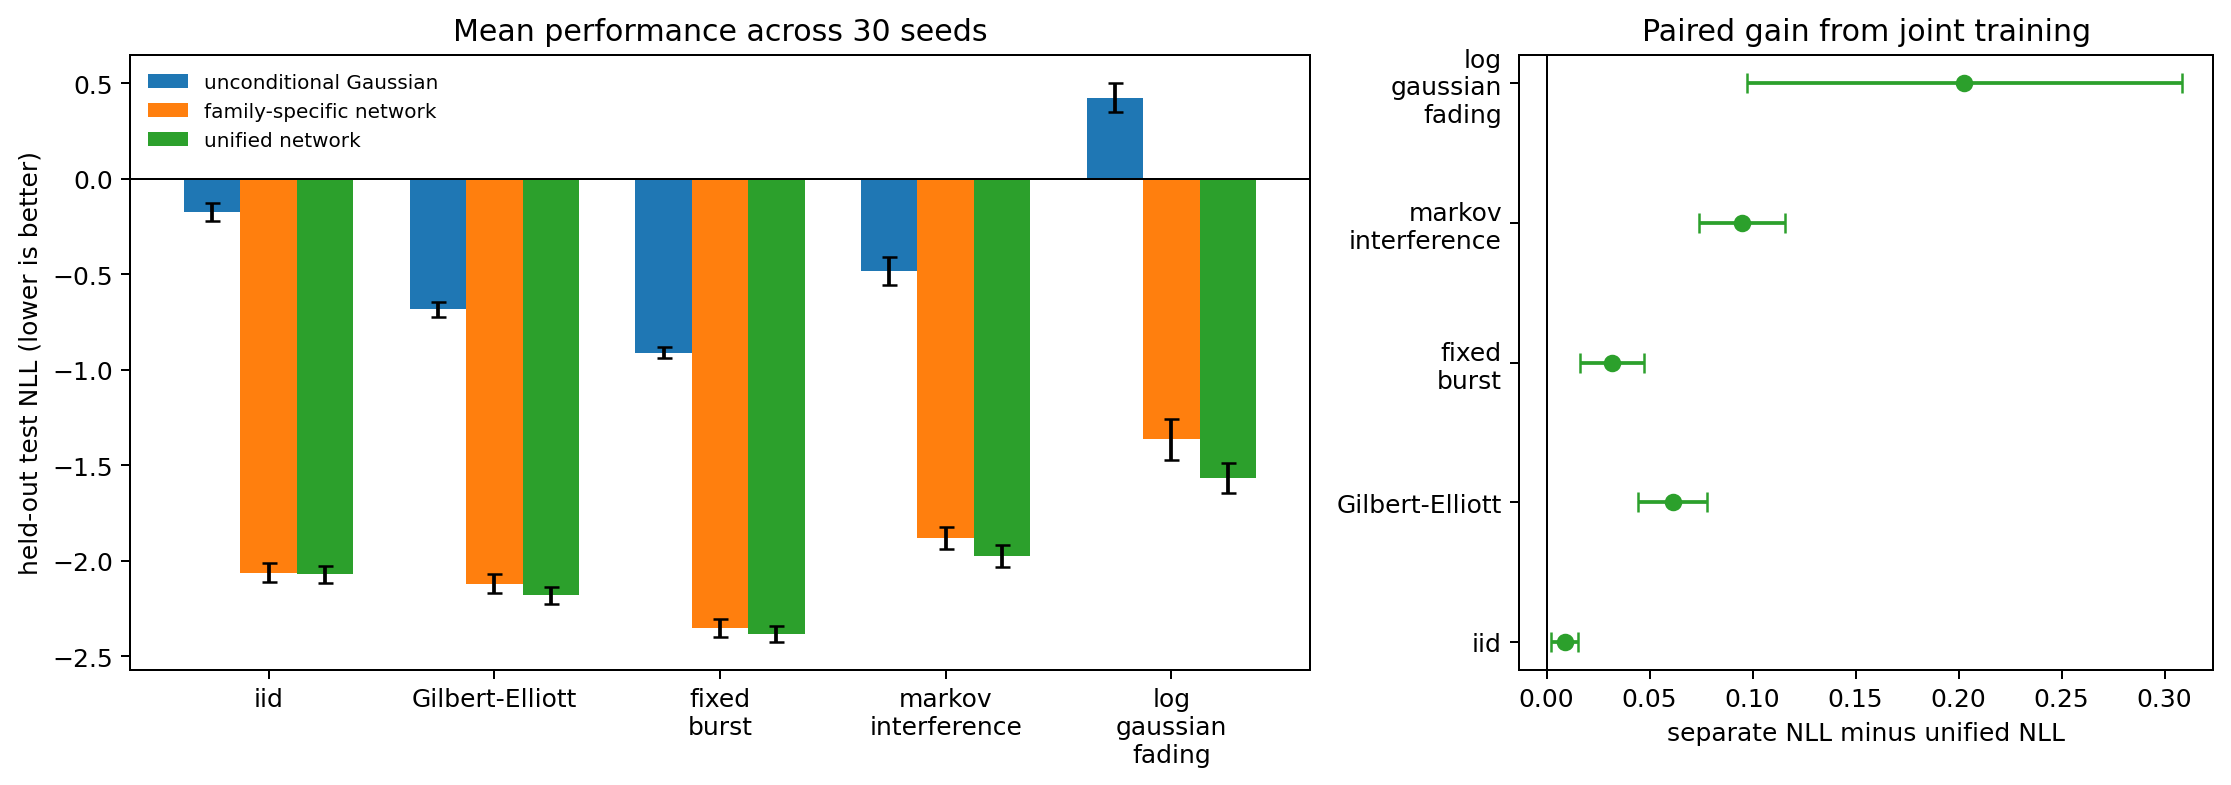
\includegraphics[width=\linewidth]{../results/repeated_benchmark/comparison_30_seeds.png}
\caption{Held-out NLL and paired joint-training gain over 30 independent seeds. Error bars are two-sided 95\% Student-$t$ confidence intervals across seeds. Lower NLL is better; positive paired gain favors joint training.}
\label{fig:results}
\end{figure}

Table~\ref{tab:results} and Figure~\ref{fig:results} compare the learned distributions. Both neural approaches sharply outperform the unconditional Gaussian reference for every family. The central comparison is between the two neural strategies.

\begin{table}[h]
\centering
\small
\caption{Held-out NLL across 30 seeds. Brackets give the 95\% confidence interval for paired gain. Gain is separate minus joint; positive values favor joint training.}
\label{tab:results}
\resizebox{\linewidth}{!}{%
\begin{tabular}{lccccr}
\toprule
Family & Unconditional & Separate MDN & Joint MDN & Paired gain & Win rate \\
\midrule
IID & $-0.1740$ & $-2.0623$ & $-2.0711$ & $0.0087$ $[0.0022,0.0153]$ & 63.3\% \\
Gilbert--Elliott & $-0.6846$ & $-2.1206$ & $-2.1818$ & $0.0612$ $[0.0443,0.0780]$ & 93.3\% \\
Fixed burst & $-0.9120$ & $-2.3515$ & $-2.3832$ & $0.0317$ $[0.0163,0.0471]$ & 73.3\% \\
Markov interference & $-0.4816$ & $-1.8796$ & $-1.9744$ & $0.0948$ $[0.0738,0.1159]$ & 100.0\% \\
Log-Gaussian fading & $0.4243$ & $-1.3640$ & $-1.5669$ & $0.2029$ $[0.0975,0.3083]$ & 76.7\% \\
\midrule
Macro average & $-0.3656$ & $-1.9556$ & $-2.0355$ & $0.0799$ $[0.0595,0.1002]$ & 96.7\% \\
\bottomrule
\end{tabular}}
\end{table}

The macro gain is 0.0799 NLL units, with a confidence interval excluding zero and a paired-test $p$-value of $7.69\times10^{-9}$. Every family-level interval also excludes zero. Gilbert--Elliott, fixed-burst, and Markov-interference contain discrete latent regimes or burst events, suggesting that shared training helps the joint MDN learn reusable mappings from state and action to multimodal telemetry.

IID gain is only 0.0087 with interval $[0.0022,0.0153]$ and $p=0.011$, so the advantage is statistically detectable but small in NLL units. The fading mean gain is much larger, 0.2029, with interval $[0.0975,0.3083]$ and $p=4.75\times10^{-4}$. Fading also has the widest gain interval, consistent with a smooth latent trajectory inducing a broader range of frame-level outcomes. Thus joint training is clearly favored in the mean, while the size of the fading benefit varies appreciably by seed.

The joint model's result is notable because it uses 12,111 parameters rather than 28,363 parameters across five separately deployed models. This is a 57.3\% reduction in total parameter storage for the tested collection. That comparison does not imply lower training cost: the joint model trains for more epochs on the combined dataset.

\section{Related Work}

\subsection{Simulation-based neural likelihoods}

The general SBI setting is well established. Cranmer, Brehmer, and Louppe survey inference with high-fidelity simulators whose likelihoods are intractable, and identify neural density estimation and simulation-guiding active learning as central developments \cite{cranmer2020frontier}. Papamakarios, Sterratt, and Murray's Sequential Neural Likelihood trains an autoregressive flow to approximate a simulator likelihood and sequentially concentrates simulations in high-posterior-density regions \cite{papamakarios2019snl}. Our implementation uses an amortized MDN over a fixed state design instead of an autoregressive flow or sequential proposal. The common idea is to learn a normalized conditional likelihood that can be combined with a prior.

Evaluation practices are equally important. Lueckmann et al. show that conclusions depend on the metric, that sequential algorithms can improve sample efficiency, and that no evaluated SBI algorithm is uniformly best \cite{lueckmann2021benchmarking}. Their benchmark motivates our grouped held-out states, repeated seeds, and direct reporting of predictive NLL. Our study remains narrower: it does not yet test posterior calibration, simulation-based calibration, classifier two-sample tests, or coverage.

Boelts et al. develop mixed neural likelihood estimation for observations containing discrete choices and continuous reaction times, then use the learned likelihood with standard posterior samplers \cite{boelts2022flexible}. That factorization directly motivates a future extension here: learn the stored binary success variable jointly with continuous reliability and effort rather than discarding it from the current target. Their application and architecture differ from ours, but they demonstrate that mixed observations need not prevent likelihood-based SBI.

\subsection{Burst channels and learned wireless channel models}

The two-state burst model traces to Gilbert's good/bad Markov channel \cite{gilbert1960capacity}; Elliott used that model to estimate coding error and retransmission behavior \cite{elliott1963estimates}. Our Gilbert--Elliott simulator preserves the two-state Markov structure but allows nonzero, state-dependent symbol-error rates in both states. The separate ON/OFF interference family has a similar latent topology but a different interpretation and parameter range.

Data-driven wireless work often learns a channel generator so that communication systems can be trained or simulated without a differentiable analytical channel. O'Shea, Roy, and West use a variational generative adversarial formulation to learn stochastic channel behavior from observations \cite{oshea2019approximating}. Ye et al. condition a channel GAN on received pilot signals and study AWGN, Rayleigh, and frequency-selective cases in an end-to-end communication system \cite{ye2020conditional}. Orekondy, Behboodi, and Soriaga learn an implicit distribution over band-limited MIMO impulse responses and evaluate power, delay, and spatial statistics on 3GPP tapped-delay-line channels \cite{orekondy2022mimogan}. These methods synthesize channel outputs or impulse responses. Our model instead assigns an explicit density to low-dimensional receiver telemetry conditional on a simulator state and action.

Generative channel models also incorporate environment context. Xia et al. combine link-state prediction with a conditional variational autoencoder that generates path losses, delays, and angles for ray-traced 28 GHz UAV channels \cite{xia2022generative}. Arvinte and Tamir learn a score for MIMO channel distributions and use posterior sampling for channel estimation, reporting simulated robustness and pilot-density results \cite{arvinte2023score}. These studies point toward higher-fidelity backends and richer observations. They do not make the current synthetic telemetry a measured propagation model, but they demonstrate practical pathways from simulator-based prototypes toward spatial, waveform, and MIMO data.

\section{Software Architecture and Reproducibility}

The package separates channel simulation, receiver measurement, dataset generation, likelihoods, and Bayesian inference. A new backend implements a small channel interface and returns an error sequence plus optional diagnostics. A new receiver implements a second interface and maps raw outcomes to observable telemetry. This separation permits later replacement of either side without changing the density-model API.

The complete repeated experiment is launched with:
\begin{verbatim}
python scripts/repeat_benchmark.py --no-resume
\end{verbatim}
It checkpoints raw seed-level rows after every seed and resumes by default. Outputs include `per\_seed.csv', aggregate CSV and JSON files, and Figure~\ref{fig:results}. Model construction, data generation, grouped splitting, training order, and simulator draws are explicitly seeded. Unit tests cover simulators, dataset splitting and reproducibility, density shapes and training, inference, and repeated-result aggregation.

\section{Limitations and Next Steps}

The strongest limitation is realism. The receiver is a stochastic analytical abstraction, and the channel backends operate on symbol-error processes rather than complex baseband waveforms. Results establish software and statistical behavior for the included simulators, not field performance. A useful next milestone is a conventional coding backend that exposes success, iterations, reliability summaries, and latency while retaining the same measurement interface.

Second, the continuous MDN does not model binary success. A mixed Bernoulli-continuous likelihood, following the general decomposition demonstrated by Boelts et al. \cite{boelts2022flexible}, would use all stored telemetry and permit success-calibrated decision objectives. Third, held-out states are interpolative draws from the training family ranges. Future tests should reserve edge ranges, entire environments, and eventually entire families to measure extrapolation and transfer.

Fourth, NLL alone does not guarantee calibrated posterior inference. Posterior predictive checks, probability-integral-transform diagnostics, expected coverage, simulation-based calibration, and comparison against non-neural conditional kernel baselines should be added. Finally, the fading result calls for a targeted capacity study covering network width, component count, full-covariance mixtures or flows, more state points, and longer frames. The existing resumable seed runner provides the base for these ablations.

\section{Conclusion}

The repository now provides an end-to-end, tested implementation of action-conditioned neural likelihood learning across five stochastic wireless channel families. A 30-seed paired experiment finds that one family-conditioned joint MDN is more parameter-efficient and improves macro-average held-out NLL over five separate MDNs. The paired mean gain is positive for every family, modest for IID errors, and largest for log-Gaussian fading. The result supports joint amortization as the default for this simulator collection, while the documented limitations make clear that mixed telemetry, calibration, out-of-distribution testing, and higher-fidelity receiver and channel backends are the appropriate next steps.

\bibliographystyle{plain}
\bibliography{references}

\end{document}
